
    \item Three vectors \( \vec{P} \), \( \vec{Q} \), and \( \vec{R} \) are shown in the figure. Let \( S \) be any point on the vector \( \vec{R} \). The distance between the points \( P \) and \( S \) is \( b|\vec{R}| \). The general relation among vectors \( \vec{P} \), \( \vec{Q} \) and \( \vec{S} \) is
        \begin{tasks}(2)
            \task \( \vec{S} = (1 - b)\vec{P} + b\vec{Q} \)
            \task \( \vec{S} = (b - 1)\vec{P} + b\vec{Q} \)
            \task \( \vec{S} = (1 - b^2)\vec{P} + b\vec{Q} \)
            \task \( \vec{S} = (1 - b)\vec{P} + b^2\vec{Q} \)
        \end{tasks}

\begin{center}
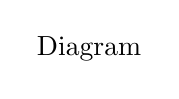
\begin{tikzpicture}
\node {Diagram};
\end{tikzpicture}
\end{center}